\documentclass[a4paper,11pt,pdf]{pacmanreport}

%%=== Aditional packages
\usepackage{xcolor}
\usepackage{pdfpages}

%%=== Local definitions
\graphicspath{{images/}{../shared_images/}}

%% ================================
%% PROJECT INFO 

\project{}
\projectid{FP7-IST-60918}
\projectstart{1 March 2013}
\duration{36}

%% ================================
%% DELIVERABLE INFO 

\title{Forming parts by manipulation}
\deliverableid{DR 2.2}
\author{Safoura Rezapour-Lakani, Justus Piater}
\address{Institute of Computer Science, University of Innsbruck}
\email{Justus.Piater@uibk.ac.at}
\headertitle{Forming Parts by Manipulation}
\headerauthor{S. Rezapour, J. Piater}

\duedate{2016-02-29}
\submissiondate{2016-02-29}
\leadpartner{UIBK}
\revision{draft}
\disseminationlevel{PU}


%% UNCOMMENT: to get the logo; if you've copied this file to a directory yearX/wpY/ then this should work
\reportlogo{pacmanlogo}


\begin{document}

\maketitle

\begin{abstract}
\noindent 
This deliverable report describes results of Task 2.3 as specified in
the DoW.  The objective of this Task is the development of methods for
influencing the formation of compositions in a hierarchical object
representation by robotic grasps of training objects.  Here we
describe a novel method that decomposes objects into graspable
regions with different grasping success probabilities,
%% JP: I do not understand the following:
%% represents objects based on different resolution of grasping,
and encodes grasping parameters and success probabilities as part of
the region representation. This representation leads to efficient and
robust grasping inference on novel objects.

%This way of integrating grasping into object representation is to the best of our knowledge a new method in object representation 
\end{abstract}


\vspace{.2em}
\hrule

\footnotesize

\tableofcontents

\normalsize

\newpage

\section*{Executive Summary}

%What does the report present? What tasks does it address? How has progress been evaluated? What previous reports does this report follow up on? 

This report presents the results of Task 2.3 on forming parts by
robotic grasping experiments. We describe an approach for representing
objects in terms of their graspable regions. Furthermore, we integrate
grasping parameters with visual object features. The detail of this
approach, which is submitted as a conference paper, is presented in
Annex~\ref{ann:wacv}.

\section*{Role of forming parts by manipulation in PaCMan}

%What role do the tasks addressed in this report play in the larger context of PaCMan? How do these tasks, how does report, contribute to achieving the overall goals for PaCMan?

There are many ways to decompose object representations hierarchically
into parts, or equivalently, to group parts hierarchically into an
object representation.  Different ways of doing so result in different
notions of parts, which differ in their practical usefulness.  One
practically-important use of a part is to grasp it.  Accordingly,
humans tend to think of objects as being composed of graspable parts.
Likewise, Task~2.3 seeks to produce methods that form compositional
representations whose parts are graspable, or more generally, that
allow a meaningful prediction of the graspability of individual parts.
We achieve this by influencing the composition by empirical
graspability.

%% DR2.2 focuses on developing a method for influencing the formation of
%% the compositional model by the grasps that are used as training
%% data. Integrating grasping into object representation ensures the
%% construction of semantically meaningful functional parts. This
%% representation plays an important role in object manipulation
%% scenarios such as grasping which is the main focus of PaCMan.

\section*{Contribution to the PaCMan scenario}

%How do the results presented in this report contribute to the PaCMan scenarios and prototypes?

As we demonstrate, forming compositions based on graspable parts
allows the transfer of grasp parameters to novel objects based on
known parts.  Moreover, the model integrates visual features and grasp
parameters into a combined, hierarchical representation, which is a
core objective of WP2.  We show that this representation is useful for
grasping objects under partial views and pose uncertainty.

\newpage

\section{Tasks, objectives, results}

\subsection{Planned work}

%What tasks was the report supposed to address? What objectives, results were these tasks to achieve? 

DR 2.2 addresses forming object parts by manipulation, corresponding
to Task~2.3 in the Description of Work.  The idea was to collect grasp
success statistics together with feature co-occurrences such that
compounds are favored that correspond to graspable parts.

Since there are multiple ways to form compositional hierarchies that
differ in their properties, a secondary idea was to allow multiple
hierarchies to coexist within the same representation, yielding a DAG
rather than a tree.


\subsection{Actual work performed}

%What does the report actually present? How have the tasks been addressed? To what extent have the intended objectives been achieved? Why, how -- or why not?

We succeeded at the construction of compositional representations in
terms of parts and their graspability.  The most recent method is
outlined in the paragraphs below.  For a detailed description of the
work performed, the reader is referred to the paper in Annex~\ref{ann}
of this deliverable.

%We were unable to pursue the idea of multiple, coexisting part
%hierarchies because of persistent difficulties with the development of
%the tree-structured compositional hierarchies in WP1.

The work on multiple coexisting hierarchies has been carried out in WP1 and is reported in DR1.3.

\subsubsection{Constructing object models from parts of diverse graspability}

We designed and implemented a method for representing objects based on
grasping. We designed a compositional object model based on graspable
and non-graspable object regions. We encoded two types of information
in the regions, (1) grasping success probabilities and (2) grasping
parameters in terms of gripper pose. Next, we brief\-ly explain our
compositional object representation. More details can be found in
Annex~\ref{ann}.

We learn our model on view-based RGB-D pointcloud data and by
performing robotic grasping experiments. Since the grasped regions of
an object are only partially visible in one view, we fused two views
in our experiments. We considered parallel, two-finger grasps. Thus,
we considered pairs of candidate points for grasping. We represent the
area enclosed by the candidate points based on gripper pose as an
ellipse.

Next, we compute grasping success probabilities based on the
sensitivity of a grasp to its precise localization. To this end, we
consider the neighboring ellipses of the grasped ellipse along the
direction of its principal axes. We then compute the area differences
between each of these neighboring ellipses and the grasped
ellipse. The differences along the principal axes and the parameters
of the ellipse itself compose our feature vector. The area change
in the neighboring ellipses, the more sensitive the grasp -- and the
less probable will generally be its success.

In order to capture different classes of grasps based on scale and
sensitivity, we perform clustering on these feature vectors. For each
cluster we compute the grasping success probability based on the
sensitivity of the cluster mean. We then merge the neighboring
ellipses which belong to the same cluster (having the same scale and
sensitivity) into a region.

\subsubsection{Inferring grasps for novel objects}
 
The first step in inferring grasps for a novel object is to obtain
candidate contact points. Based on two-finger
grasps during training, normal vectors at contact points tend to be
collinear. The next step is to fit ellipses to the candidate pairs and
compute area changes with respect to their neighbors which constructs
our feature vector. This feature vector is matched to our learned
clusters, and the most probable cluster is selected. The sensitivity
of the ellipse can be easily computed from its matched cluster. We
then merge the neighboring ellipses which belong to the same cluster
into a region. This gives us a segmentation based on graspability.
For grasping purpose, we select the least sensitive and most probable
regions. Furthermore, we select only the middle ellipse inside each
region for grasping.

As can be seen, this representation has two benefits. For one, there
is almost no computation time for gripper pose since it is encoded in
the ellipse itself. For another, grasp selection is done in a very
efficient way. The object is segmented into regions which have the
same grasping success probability. This reduces the search space for
finding graspable spots in an object.

%Thus, reducing search space instead of each pairs of candidates to regions. Furthermore, the most probable regions are explored first which is very robust and efficient.

\subsection{Relation to the state-of-the-art}

%How are the obtained results related to the state-of-the-art? 

The main contributions of the results achieved for Task 2.3 lie in a
novel object representation based on grasping and encoding grasping
parameters directly in the object representation, without the need to
compute them separately. Furthermore, the regions are distinctive for
the grasping task because they encode the grasp sensitivity.

The main difference from other part-based grasping methods such as the
work discussed by Stein et al.~\cite{lccp-grasp} is the benefit of
learning object regions by way of grasping rather than offline
segmentation. This provides us with regions that are by construction
suitable for grasping. Additionally, there is no need to compute
object pose for computing gripper
pose~\cite{saxena_grasp_novel_objects} which gives our approach a
computational advantage.

Furthermore, we find an appropriate level of granularity for
decomposition. To be more precise, instead of assigning grasps to a
small set of object points (\emph{patches})
\cite{saxena_deep_grasps,grasping_ng,grasping_mrf,kopicki2015a} which
incurs a large search space, or to the object level which does not
lend itself to generalization, our decomposition provides us with more
distinctive object regions, which is robust and efficient.

\bibliographystyle{ieeetr}
\bibliography{../shared_bibliography/abbreviations,./bibliography/DR22}

\newpage

\appendix
\section{Annexes}
\label{ann}

% Which papers / articles are included in the report? Mention titles,
% authors, publication info; abstract; and a one-liner relating the
% publication back to the discussion on actual work performed.

%\subsection{Article: Object Decomposition based on Graspability}
\subsection{Article: Object Representation based on Grasping}
\label{ann:wacv}

%\textbf{\textcolor{red}{This will be replaced by a new paper,
 %   currently in preparation for submission to IROS 2016.}}

%\begin{description}
%\item[Authors] Safoura Rezapour Lakani, Bj\"{o}rn Ommer, Antonio
 % J. Rodr\'{i}guez-S\'{a}nchez and, Justus Piater
%\item[Info] submitted to the IEEE Winter Conference on Applications of
 % Computer Vision (WACV), 2016
%\item[Abstract] Objects are composed of a configuration of parts which
 % are mostly designed for a certain functionality. For example a
  %spatula is designed for scooping through a grasp from the
 % handle. Therefore, recognizing and representing functionalities into
  %object representation is of a great importance. This representation
  %must provide us with an efficient inference of
  %functionalities. Therefore, the representation must be
  %discriminative enough. We introduce here a novel compositional model
  %based on grasping functionality. Objects are represented based on
  %graspability of their regions. Moreover, the grasps and their
  %robustness are encoded into the representation. This allows us for
  %efficient and robust search for graspability on objects. We
  %evaluated our method in a robotic grasping scenario and achieved a
  %promising accuracy for novel objects.
%\item[Relation with the Deliverable]\hfill This paper reports work
 % done under\\ Task~2.3 by introducing a method for representing
  %objects based on robotic grasping experiments.
%\item[Attachment] (following pages)
%\end{description}

\begin{description}
\item[Authors] Safoura Rezapour Lakani, Bj\"{o}rn Ommer, Antonio J. Rodr\'{i}guez-S\'{a}nchez, Sandor Szedmak, Senka Krivic and Justus Piater
\item[Info] in preperation for the IEEE/RSJ International Conference on Intelligent Robots and Systems (IROS), 2016
\item[Abstract] Most human-made objects are composed of a configuration of parts whose
design serves a certain functionality. As an example, a spatula is
designed for scooping; the handle is the part of the object designed
to grasp it in order to perform that operation. The functionality of
an object's part and also the object can be related to its visual
representation. In this paper we follow on that idea in order to infer
the functionality of an object through its representation by parts.
The focus is on graspable human-made objects; thus, the object
representation is related to their graspable characteristics.
Our evaluation on a robotic grasping scenario shows that our approach
is efficient and robust as well as transferable to previously unseen,
novel objects.
\item[Relation with the Deliverable]\hfill This paper reports work
  done under\\ Task~2.3 by introducing a method for representing
  objects based on robotic grasping experiments.
\item[Attachment] (following pages)
\end{description}

%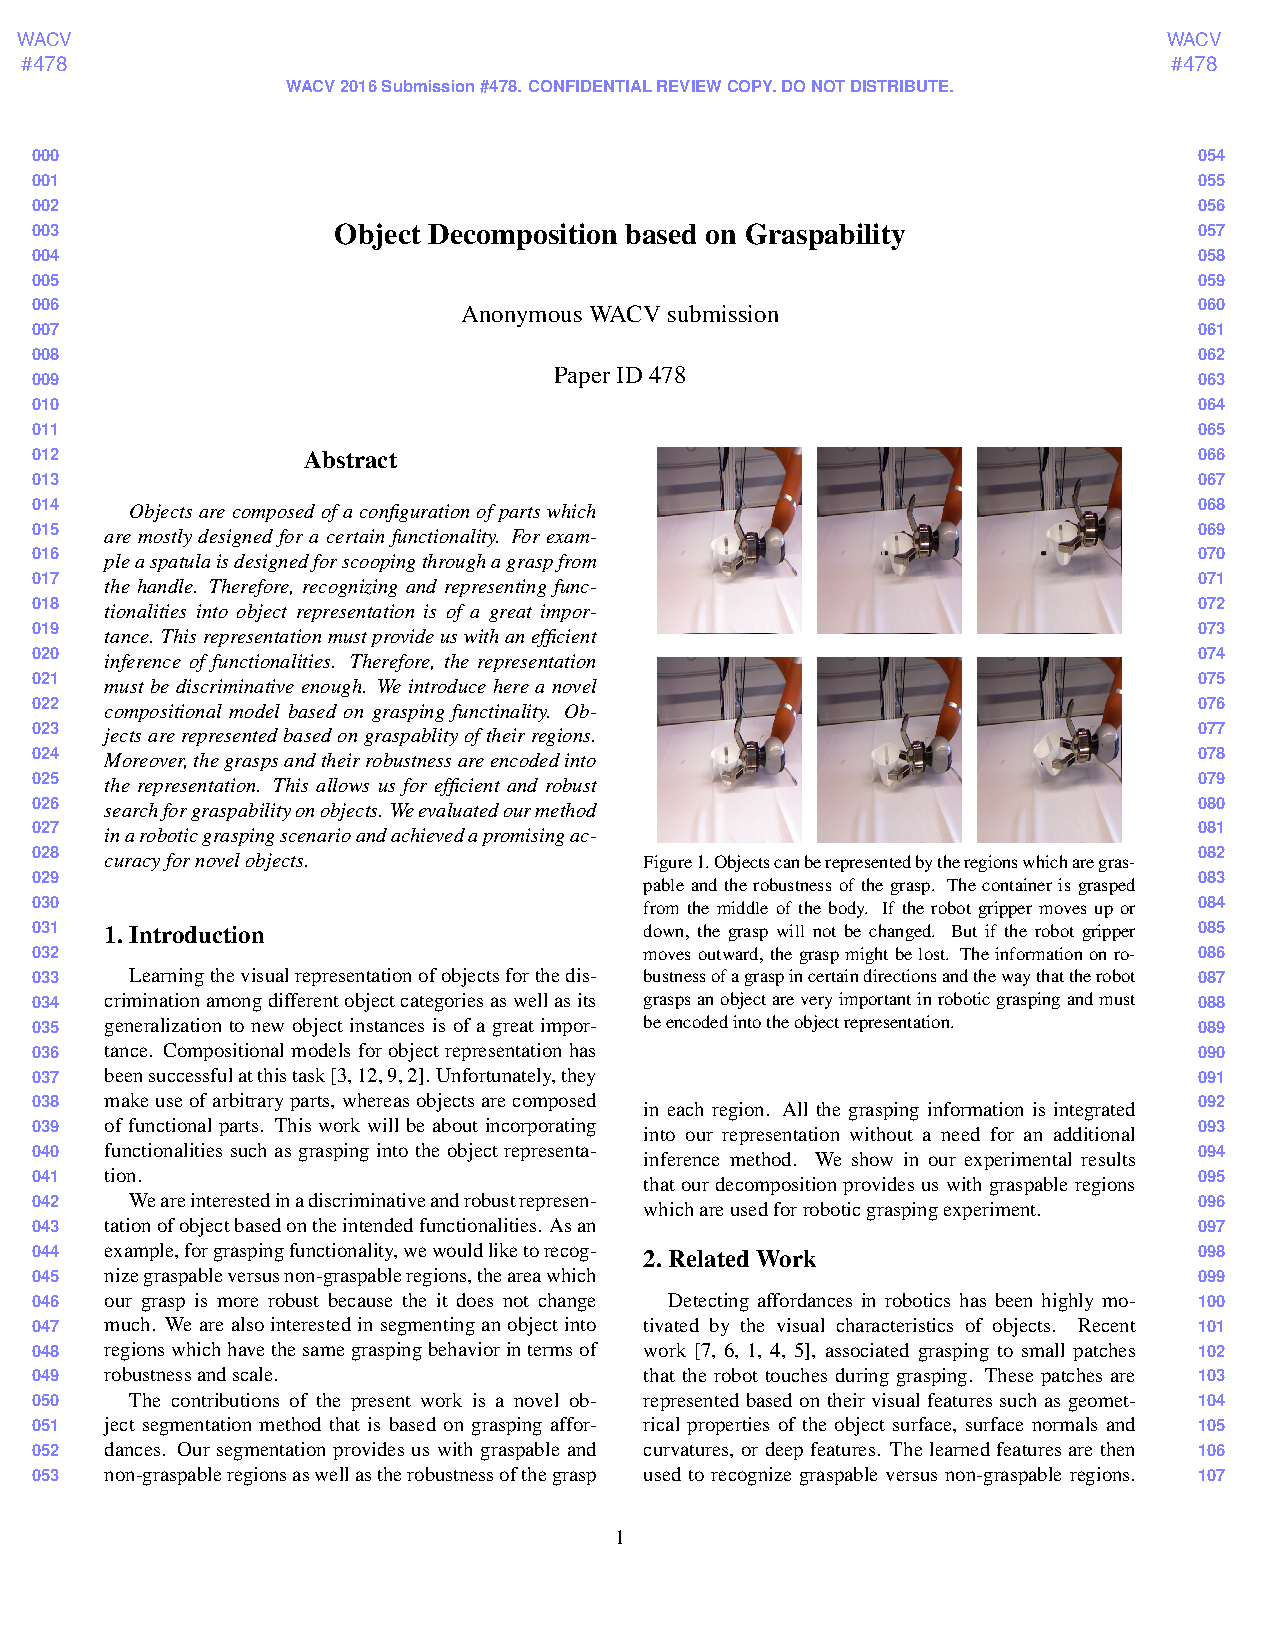
\includepdf[pages=-]{./attachedPapers/rezapouretal-wacv2016.pdf}
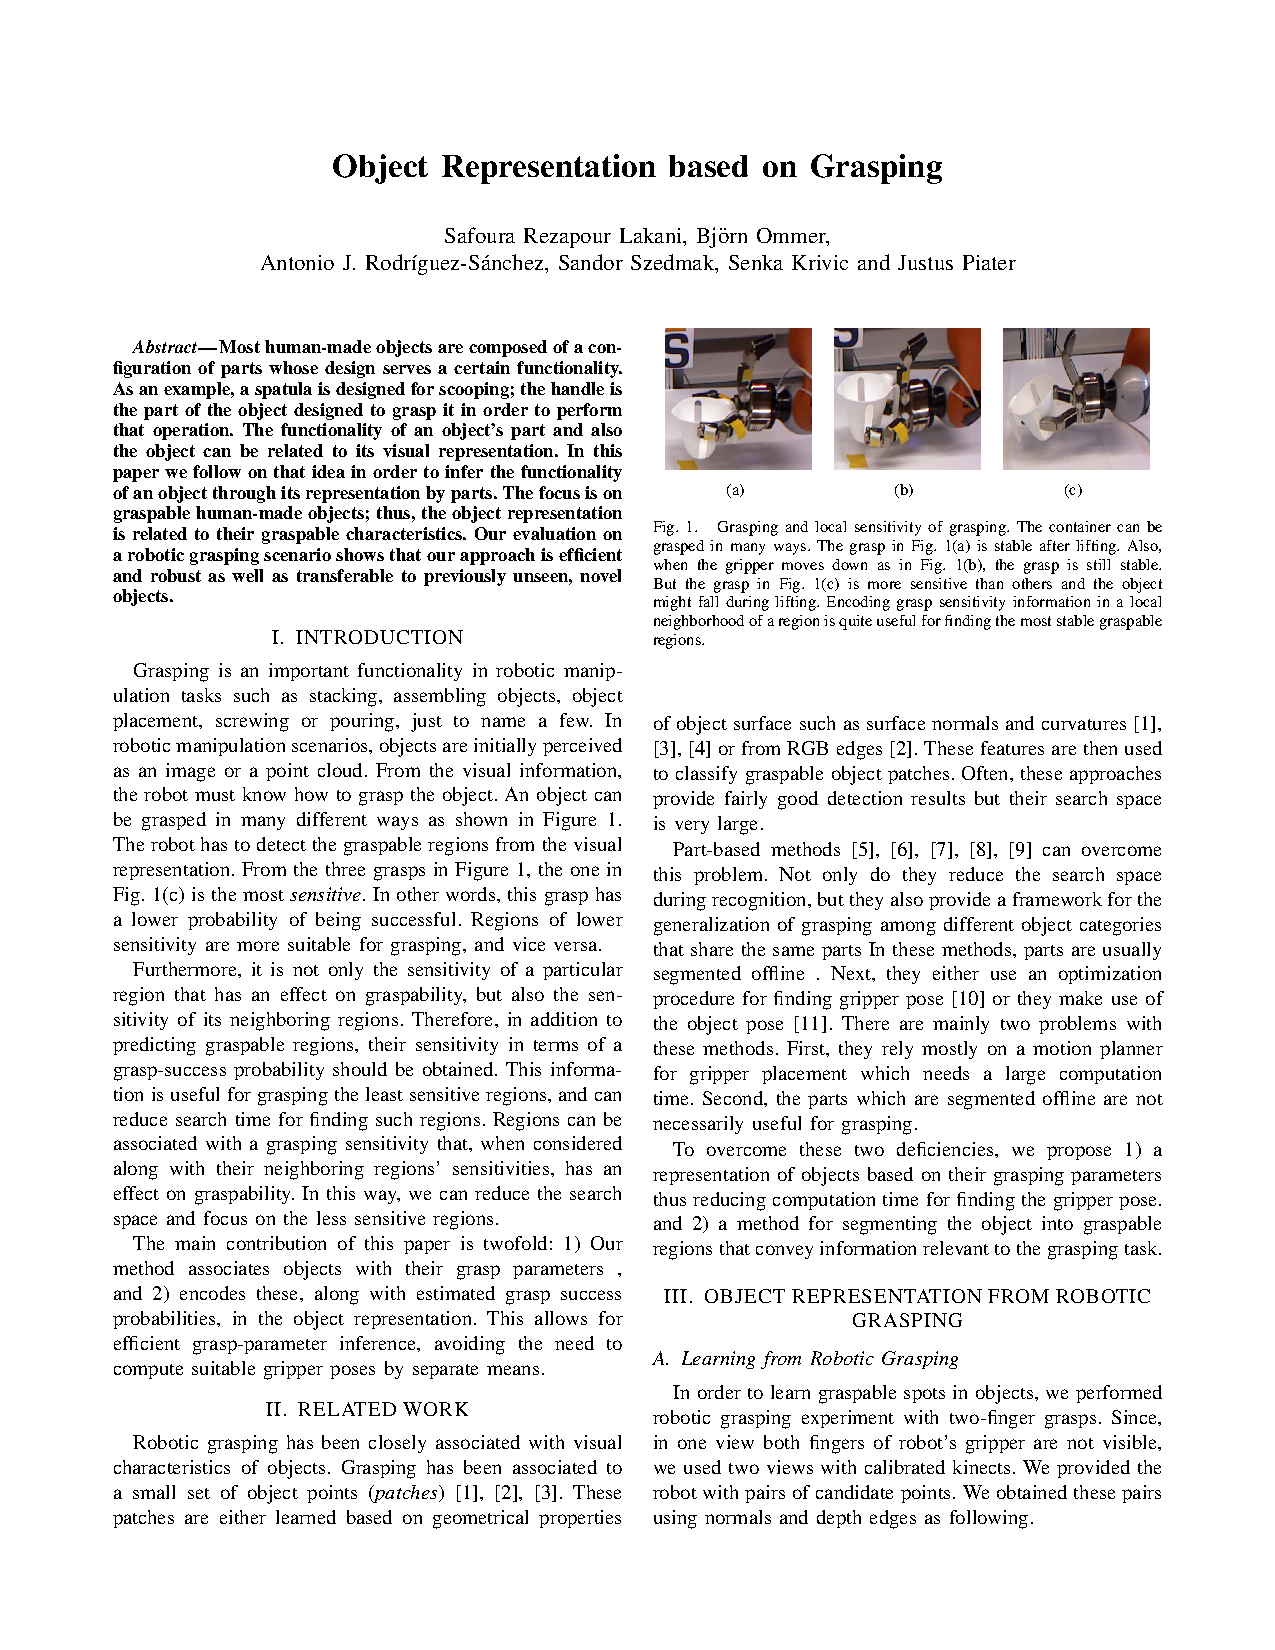
\includepdf[pages=-]{./attachedPapers/rezapouretal-iros2016.pdf}

\end{document}
